\documentclass[12pt,a4paper,ngerman]{article}
\usepackage{stylesheet}
\begin{document}
\TUHeader                          %  Bitte Ausfüllen!!!
%----------------------------
{Übung F: Übertragungsverhalten nachrichtentechnischer Systeme}                       %  Übungstitel
%----------------------------
{25.11.2014}                        %  Übungsdatum
%----------------------------
{05}                            %  Gruppen-Nr.
%----------------------------
{Thomas Neff}                   % Name des Protokollführers
%----------------------------
{
1.~Daniel Freßl, 1230028\\
2.~Thomas Neff, 1230319\\                    %  Übungsteilnehmer
3.~Thomas Pichler, 1230320 \\                   %  ...bei <4 Teilnehmer auskommentieren
4.~Martin Winter, 1130688\\
5.~Bernadette Schreyer, 1073076\\
}
%----------------------------
{Ao.Univ.-Prof. Dipl.-Ing. Dr. techn. Erich Leitgeb}
{Max Henkel}                          %  Betreuer
%----------------------------
{Graz}                              %  Ort der Protokollerstellung
{\today}                            %  Datum Protokollerstellung




\pagebreak
  
\tableofcontents
  
\pagebreak

%-------------------------------------------------------------------------------
%
% Beginn des Protokolls
%
%-------------------------------------------------------------------------------

\section{Rückwirkungsfreie Messung des H-Feldes zweier PCD-Schleifenantennen mit unterschiedlichen Güten}
\subsection{Aufgabenstellung}
Bei dieser Aufgabe sollten zwei Antennen mit unterschiedlicher Güte (5, 50) miteinander verglichen werden. Dazu soll die magnetische Feldstärke in Abhängigkeit von der Entfernung zur Antenne gemessen werden (in 5mm Schritten, von 0 bis 14cm).\\
Weiters soll die Anstiegszeit des Sendesignals, von 10\% auf 90\% der Trägersignalamplitude, für beide Antennen bestimmt werden.

\subsection{Messaufbau}
Für den Messaufbau wurde ein speziell dafür modifizierter RFID-Reader mit regelbarer Ausgangsamplitude verwendet. Dieser wurde an einen Computer und einen Verstärker angeschlossen. Zwischen Verstärker und zu vermessender Antenne wurde ein Dämpfer (6db) eingebaut.\\
Die Antenne und die zur Messung verwendete Referenzspule wurden in einen verstellbaren Distanzhalter platziert. Zur Messung wurde die Referenzspule an ein Oszilloskop angeschlossen.

\subsection{Tabellen}
\begin{table}[H]
\begin{center}
\begin{tabular}{ |c|c|c|c|c| }
  \hline
     & Q=50 & Q=5 & Q=50 & Q=5\\

    Distanz & $U_i(pp)$ & $U_i(pp)$ & H(rms) & H(rms)\\

  [cm] & [V] & [V] & [A/m] & [A/m] \\
  \hline
  0 & $2.9$ & $0.894$ & $3.167$ & $0.976$ \\
  \hline
  $0.5$ & $2.75$ & $0.863$ & $3.003$ & $0.942$ \\
  \hline
  $1$ & $2.61$ & $0.813$ & $2.85$ & $0.888$ \\
  \hline
  $1.5$ & $2.44$ & $0.756$ & $2.664$ & $0.826$ \\
    \hline
  $2$ & $2.25$ & $0.706$ & $2.457$ & $0.771$ \\
    \hline
  $2.5$ & $2.06$ & $0.637$ & $2.249$ & $0.696$ \\
    \hline
  $3$ & $1.89$ & $0.584$ & $2.064$ & $0.638$ \\
    \hline
  $3.5$ & $1.7$ & $0.531$ & $1.86$ & $0.579$\\
    \hline
  $4$ & $1.55$ & $0.481$ & $1.69$ & $0.525$ \\
    \hline
  $4.5$ & $1.39$ & $0.434$ & $1.52$ & $0.474$ \\
    \hline
  $5$ & $1.25$ & $0.425$ & $1.37$ & $0.464$ \\
    \hline
  $5.5$ & $1.13$ & $0.425$ & $1.23$ & $0.464$ \\
     \hline
  $6$ & $1.01$ & $0.425$ & $1.102$ & $0.464$ \\
      \hline
  $6.5$ & $0.92$ & $0.425$ & $1.004$ & $0.464$ \\ 
      \hline
  $7$ & $0.82$ & $0.425$ & $0.895$ & $0.464$ \\
      \hline
  $7.5$ & $0.75$ & $0.425$ & $0.819$ & $0.464$ \\
      \hline
  $8$ & $0.68$ & $0.425$ & $0.743$ & $0.464$ \\
      \hline
  $8.5$ & $0.62$ & $0.425$ & $0.677$ & $0.464$ \\
      \hline
  $9$ & $0.55$ & $0.425$ & $0.6$ & $0.464$ \\
      \hline
  $9.5$ & $0.5$ & $0.425$ & $0.546$ & $0.464$ \\
      \hline
  $10$ & $0.46$ & $0.425$ & $0.502$ & $0.464$ \\
      \hline
  $10.5$ & $0.41$ & $0.425$ & $0.448$ & $0.464$ \\
      \hline
  $11$ & $0.38$ & $0.425$ & $0.415$ & $0.464$ \\
      \hline
  $11.5$ & $0.35$ & $0.425$ & $0.382$ & $0.464$ \\
      \hline
  $12$ & $0.32$ & $0.425$ & $0.349$ & $0.464$ \\
      \hline
  $12.5$ & $0.29$ & $0.425$ & $0.317$ & $0.464$ \\
      \hline
  $13$ & $0.29$ & $0.425$ & $0.317$ & $0.464$ \\
      \hline
  $13.5$ & $0.29$ & $0.425$ & $0.317$ & $0.464$ \\
        \hline
  $14$ & $0.29$ & $0.425$ & $0.317$ & $0.464$ \\  \hline
\end{tabular}
\caption{Test}
\end{center}
\label{tab:1}
\end{table}
\pagebreak
\subsection{Formeln}
Diese Formel stellt den Zusammenhang zwischen induzierter Spannung und Feldstärke dar. Die verwendeten Parameter sind $f_r = 13,56$MHz, $\mu_0 = 4\pi \cdot 10^{-7}\frac{As}{Vm}$, $\mu_r = 1$ und $A = 0,072 \cdot 0,042\ mm^2$.
\begin{equation}
U_{ind} = 2\pi \cdot f_r \cdot \mu_0 \cdot \mu_r \cdot H \cdot A
\end{equation}

Zusammenhang zwischen Spitze-Spitze-Spannung und dem Effektivwert der Spannung.
\begin{equation}
U_{pp} = \sqrt{2}  \cdot 2 \cdot U_{ind}
\end{equation}

\subsection{Berechnungsbeispiele}
Die Werte für das Berechnungsbeispiel wurden aus der Tabelle \ref{tab:1} Zeile 1 entnommen.
\begin{equation}
U_{ind} = \frac{U_{pp}}{\sqrt{2}  \cdot 2} = \frac{2,9V}{\sqrt{2}  \cdot 2} = 1,025V
\end{equation}

\begin{gather}
H = \frac{U_{ind}}{2\pi \cdot f_r \cdot \mu_e \cdot \mu_r \cdot A} = \\
\frac{1,025V}{2\pi \cdot 13,56MHz \cdot 4\pi \cdot 10^{-7}\frac{As}{Vm} \cdot 1 \cdot 0,072mm \cdot 0,042mm} = 3,167\frac{A}{m}
\end{gather}

\subsection{Diagramme}
\begin{figure}[H]
\centering
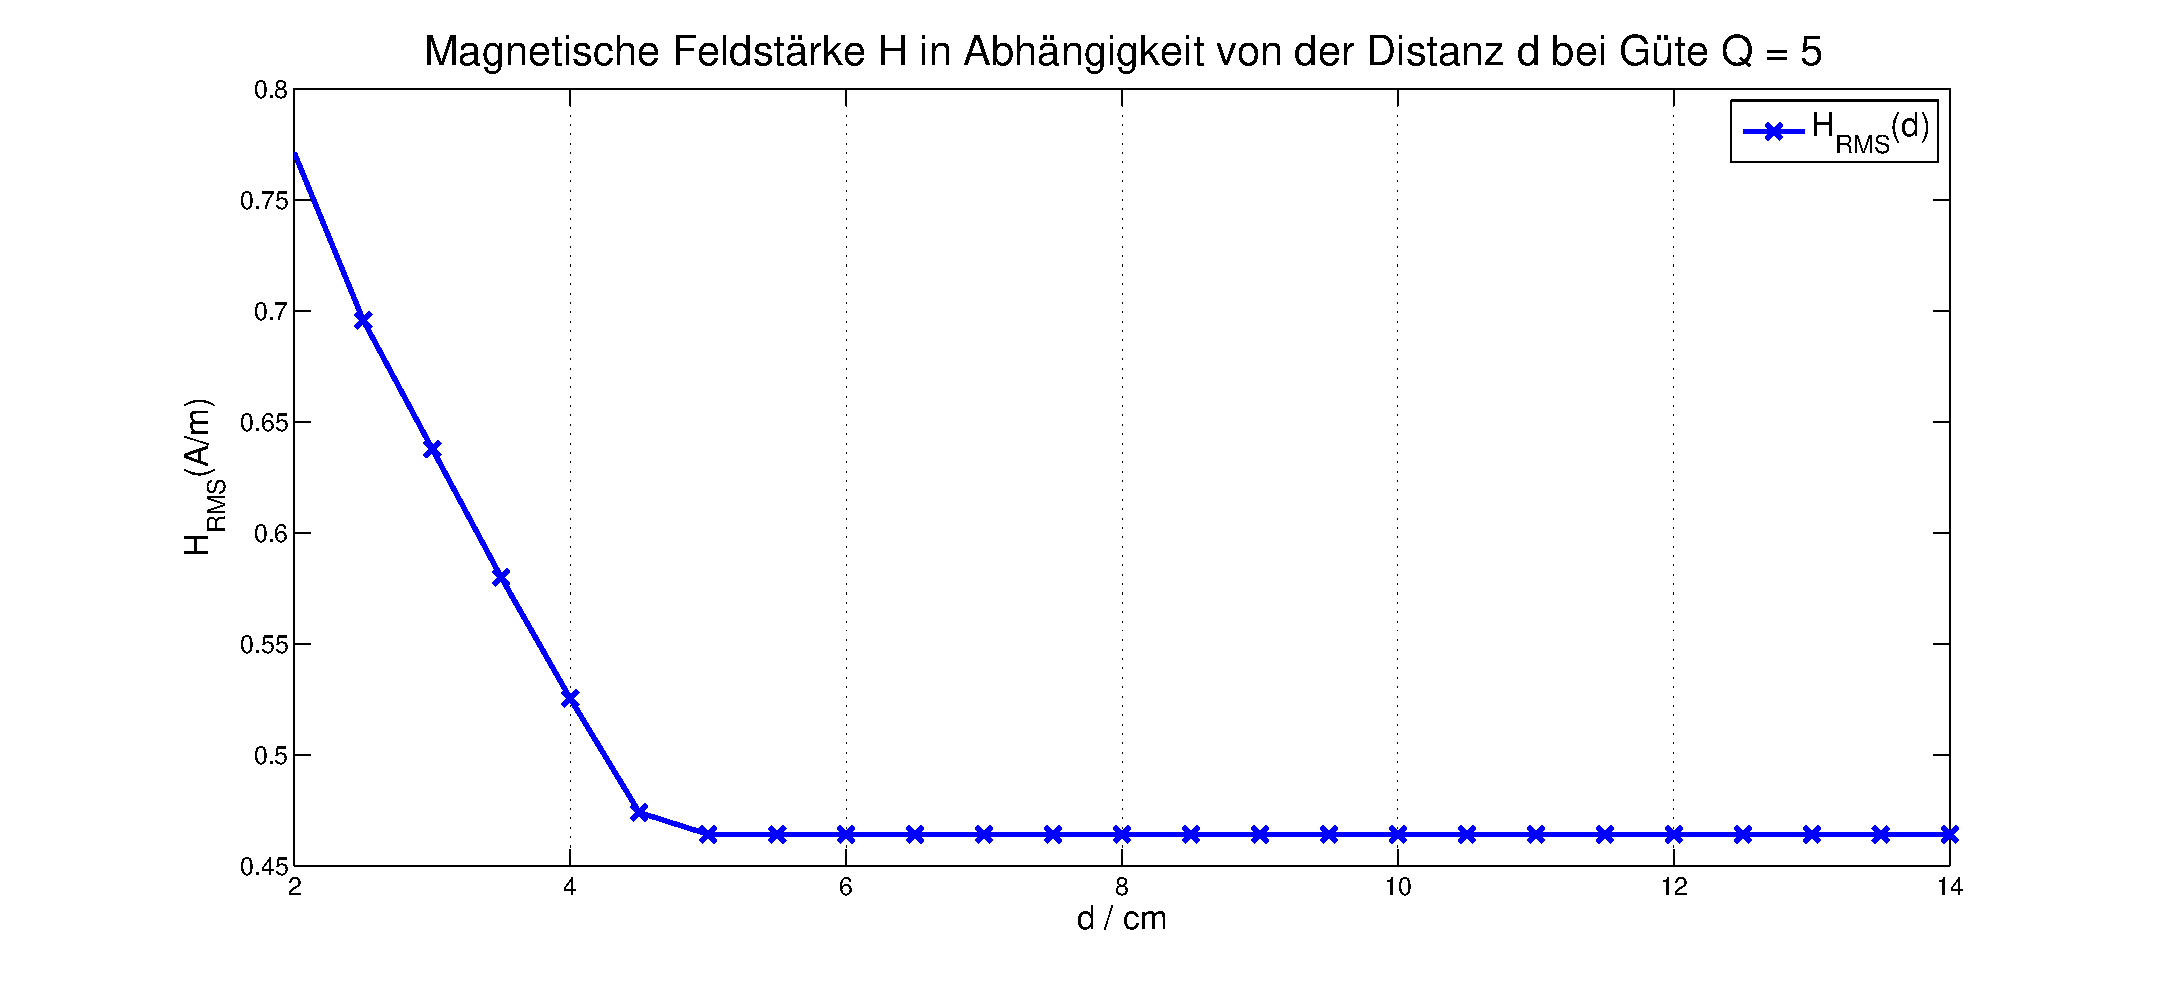
\includegraphics[width=0.9\textwidth]{figures/a1_q5.eps} 
\caption{Verlauf der Feldstärke über die Entfernung für Q = 5 und Q = 50}
\label{fig:1_q5}
\end{figure}

\begin{figure}[H]
\centering
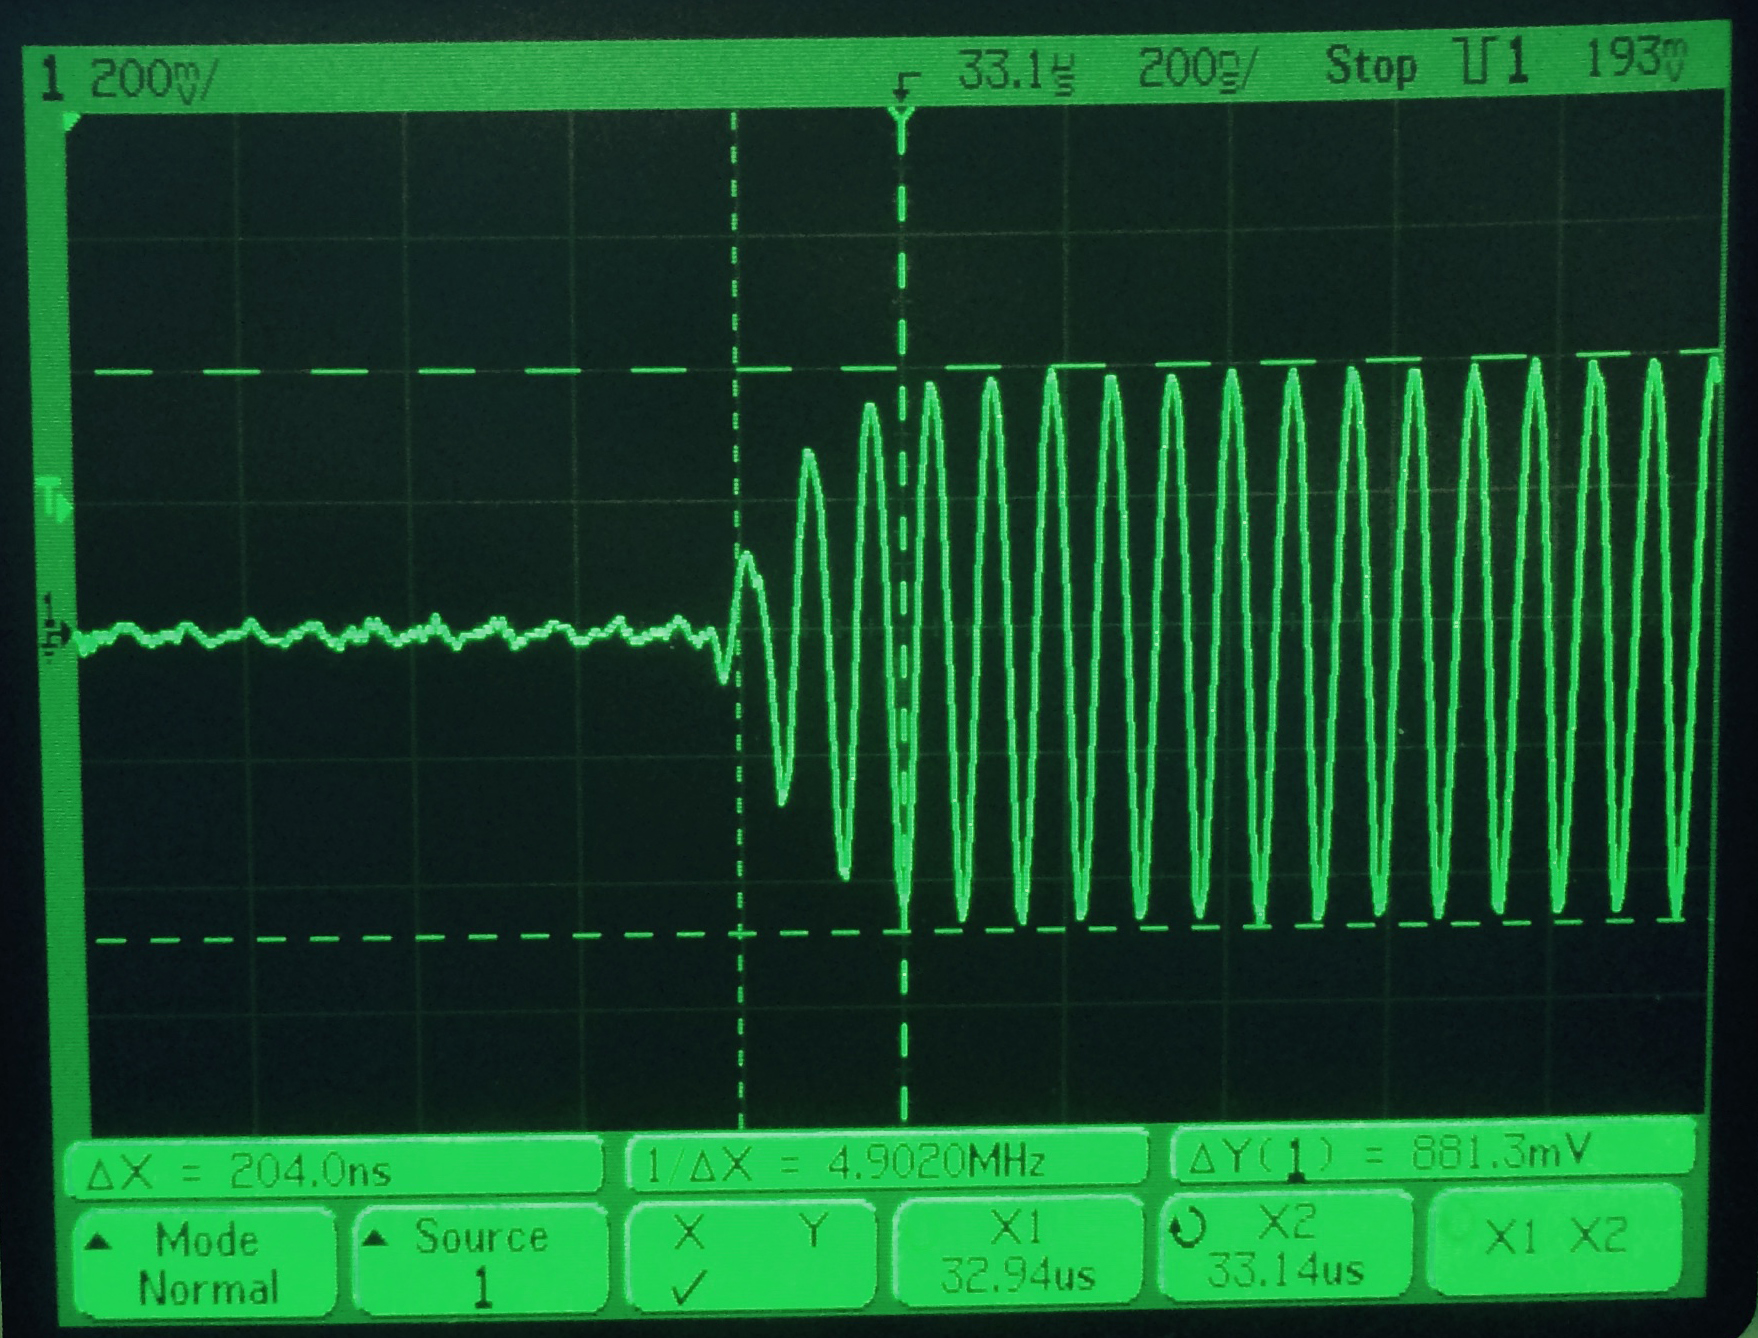
\includegraphics[width=0.9\textwidth]{figures/Anstiegq5.jpg} 
\caption{Messung der Anstiegszeit der Antenne mit Q = 5 am Oszilloskop}
\label{fig:1_anstieg}
\end{figure}

\subsection{Geräteliste}
\begin{itemize}
\item Computer
\item Reader: Labor-RFID-Reader
\item Verstärker: Amplifier Research Model 75A250
\item Dämpfer: 6dB
\item Antennen: PCD-Schleifenantennen mit Q=5 und Q=50
\item 
\end{itemize}
\pagebreak
\subsection{Diskussion}
Bei dieser Übung wurde jeweils eine Antenne (mit der Güte Q=5, Q=50) in den Aufbau eingesetzt und angeschlossen. Es wurde nur das Trägersignal ohne zusätzliche Information übertragen und mit der Referenzspule gemessen. Die Entfernung der Referenzspule zur Antenne wurde mit 5mm Schritten von 0cm auf 14cm verändert. Mit dem Oszilloskop wurde die Peak-Peak-Spannung gemessen.\\
Diese Spannung kann mit den oben angeführten Formeln in die magnetische Feldstärke umgerechnet werden. Bei der Umrechnung ist zu beachten, das die magnetische Feldstärke als Effektivwert angegeben werden soll und die Spannung als Spitze-Spitze-Wert gemessen wird.\\
Die gemessenen und berechneten Werte wurden in einem Diagramm (Abbildung \ref{fig:1_q5}) dargestellt.\\
Die magnetische Feldstärke ist bei der Antenne mit der Güte Q=50 bis zu einer Entfernung von 10cm höher.\\
\\
Zur Messung der Anstiegszeit wurde beim Oszilloskop der Single-Shot-Modus und Triggern an der fallenden Flanke mit nachfolgender Pause von $1,5\mu s$ eingestellt.\\
Der Reader wurde über die Reader-Software am Computer zum Senden eines Lesebefehls veranlasst, welcher an der Referenzspule und somit am Oszilloskop die zum Triggern benötigte negative Flanke und nachfolgende Pulsbreite (Pause) erzeugt.\\
Nach dieser Pause steigt die Amplitude des Signals wieder auf die Amplitude des Trägersignals an. Die Zeit für diesen Anstieg von 10\% auf 90\% der Signalamplitude wurde mittels Marker am Oszilloskop gemessen.\\
\begin{itemize}
\item Antenne Q = 50: $1,24\mu s$
\item Antenne Q = 5:  $204ns$
\end{itemize}
Aus diesen Werten ist ersichtlich, das die Anstiegszeit für höhere Güten größer wird. Somit kann mit Antenne mit höherer Güte zwar eine größere Reichweite aber eine geringere Datenrate erzielt werden.


\pagebreak



\section{Messung der H-Feldstärke über der Frequenz bei unterschiedlichen Antennengüten}
\subsection{Aufgabenstellung}
Bei dieser Aufgabe soll der Frequenzgang beider Antennen (Q = 5, Q = 50) von 12MHz bis 15MHz aufgenommen werden.\\

\subsection{Messaufbau}
Als Signalquelle 

\subsection{Tabellen}
\begin{table}[H]
\begin{center}
\begin{tabular}{ |c|c|c|c|c| }
  \hline
     & Q=50 & Q=5 & Q=50 & Q=5\\

    Frequenz & $U_i(pp)$ & $U_i(pp)$ & H(rms) & H(rms)\\

  [MHz] & [V] & [V] & [A/m] & [A/m] \\
  \hline
  12 & $0.363$ & $0.5$ & $0.396$ & $0.546$ \\
  \hline
  $12.2$ & $0.425$ & $0.575$ & $0.464$ & $0.628$ \\
  \hline
  $12.4$ & $0.5$ & $0.6$ & $0.546$ & $0.655$ \\
  \hline
  $12.6$ & $0.784$ & $0.813$ & $0.856$ & $0.888$ \\
    \hline
  $12.8$ & $1$ & $0.844$ & $1.092$ & $0.922$ \\
    \hline
  $13$ & $1.3$ & $0.869$ & $1.419$ & $0.949$ \\
    \hline
  $13.2$ & $1.78$ & $0.887$ & $1.944$ & $0.969$ \\
     \hline
  $13.25$ & $1.97$ & $0.894$ & $2.151$ & $0.976$ \\ 
    \hline
  $13.3$ & $2.14$ & $0.9$ & $2.337$ & $0.983$ \\
    \hline
  $13.35$ & $2.31$ & $0.906$ & $2.523$ & $0.989$ \\
    \hline
  $13.4$ & $2.5$ & $0.906$ & $2.73$ & $0.989$ \\
    \hline
  $13.45$ & $2.64$ & $0.906$ & $2.883$ & $0.989$ \\
    \hline
  $13.5$ & $2.73$ & $0.913$ & $2.981$ & $0.997$ \\
     \hline
  $13.55$ & $2.76$ & $0.913$ & $3.014$ & $0.997$ \\
      \hline
  $13.6$ & $2.7$ & $0.913$ & $2.948$ & $0.997$ \\ 
      \hline
  $13.65$ & $2.61$ & $0.919$ & $2.85$ & $1.004$ \\
      \hline
  $13.7$ & $2.45$ & $0.925$ & $2.675$ & $1.01$ \\
      \hline
  $13.75$ & $2.31$ & $0.925$ & $2.523$ & $1.01$ \\
      \hline
  $13.8$ & $2.14$ & $0.925$ & $2.337$ & $1.01$ \\
      \hline
  $14$ & $1.59$ & $0.925$ & $1.736$ & $1.01$ \\
      \hline
  $14.2$ & $1.23$ & $0.925$ & $1.343$ & $1.01$ \\
      \hline
  $14.4$ & $1.02$ & $0.919$ & $1.114$ & $1.004$ \\
      \hline
  $14.6$ & $0.86$ & $0.906$ & $0.939$ & $0.989$ \\
      \hline
  $14.8$ & $0.734$ & $0.9$ & $0.802$ & $0.983$ \\
      \hline
  $15$ & $0.653$ & $0.887$ & $0.713$ & $0.987$ \\
      \hline
\end{tabular}
\caption{Test}
\end{center}
\end{table}
\subsection{Formeln}

\subsection{Berechnungsbeispiele}


\pagebreak
\subsection{Diagramme}
%\begin{figure}[H]
%\centering
%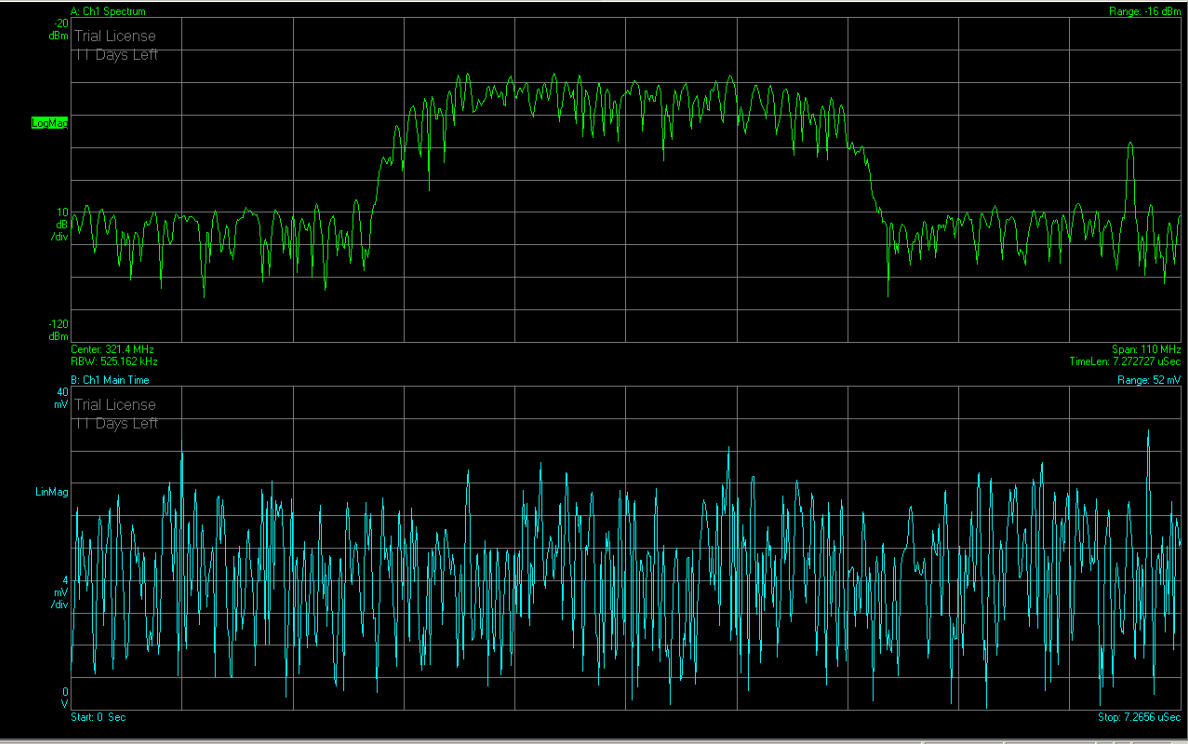
\includegraphics[width=0.9\textwidth]{figures/Aufgabe2_16QAM_1.jpg} 
%\caption{Spektrum und zeitlicher Verlauf des empfangenen 16-QAM modulierten Signals}\label{fig:aufg2_16QAM_spec}
%\end{figure}


\subsection{Diskussion}

\pagebreak



\section{Arbeitsbereich eines Lesegerätes}
\subsection{Aufgabenstellung}

\begin{itemize}
\item ???.
\end{itemize}


\subsection{Tabellen}
\begin{table}
\begin{center}
\begin{tabular}{ |c|c|c| }
  \hline

    H(rms)) & $U_i(pp) am Scope$ & $U_i(pp) am Transponder$\\

	[A/m] & [V] & [V] \\
  \hline
  0 & $0$ & $0$\\
  \hline
  $0.498$ & $0.456$ & $0.982$ \\
  \hline
  $0.997$ & $0.913$ & $1.933$\\
  \hline
  $1.4677$ & $1.344$ & $3.154$\\
    \hline
  $1.9656$ & $1.8$ & $4.21$\\
    \hline
  $2.4352$ & $2.23$ & $5.26$ \\
    \hline
  $2.9375$ & $2.69$ & $6.29$\\
     \hline
  $3.4835$ & $3.19$ & $7.46$ \\ 
    \hline
  $3.9421$ & $3.61$ & $8.5$  \\
    \hline
  $4.4663$ & $4.09$ & $9.5$  \\
    \hline
  $5.0123$ & $4.59$ & $10.52$  \\
    \hline
  $5.4928$ & $5.03$ & $11.55$  \\
    \hline
  $5.9733$ & $5.47$ & $12.55$ \\
     \hline
  $6.4537$ & $5.91$ & $13.53$ \\
      \hline
  $6.9233$ & $6.34$ & $14.55$ \\ 
      \hline
  $7.4038$ & $6.78$ & $15.56$  \\
      \hline
  $7.8515$ & $7.19$ & $16.5$  \\
      \hline 
\end{tabular}
\caption{Test}
\end{center}
\end{table} 
\subsection{Formeln}

\subsection{Berechnungsbeispiele}


\pagebreak
\subsection{Diagramme}
\begin{figure}[H]
\centering
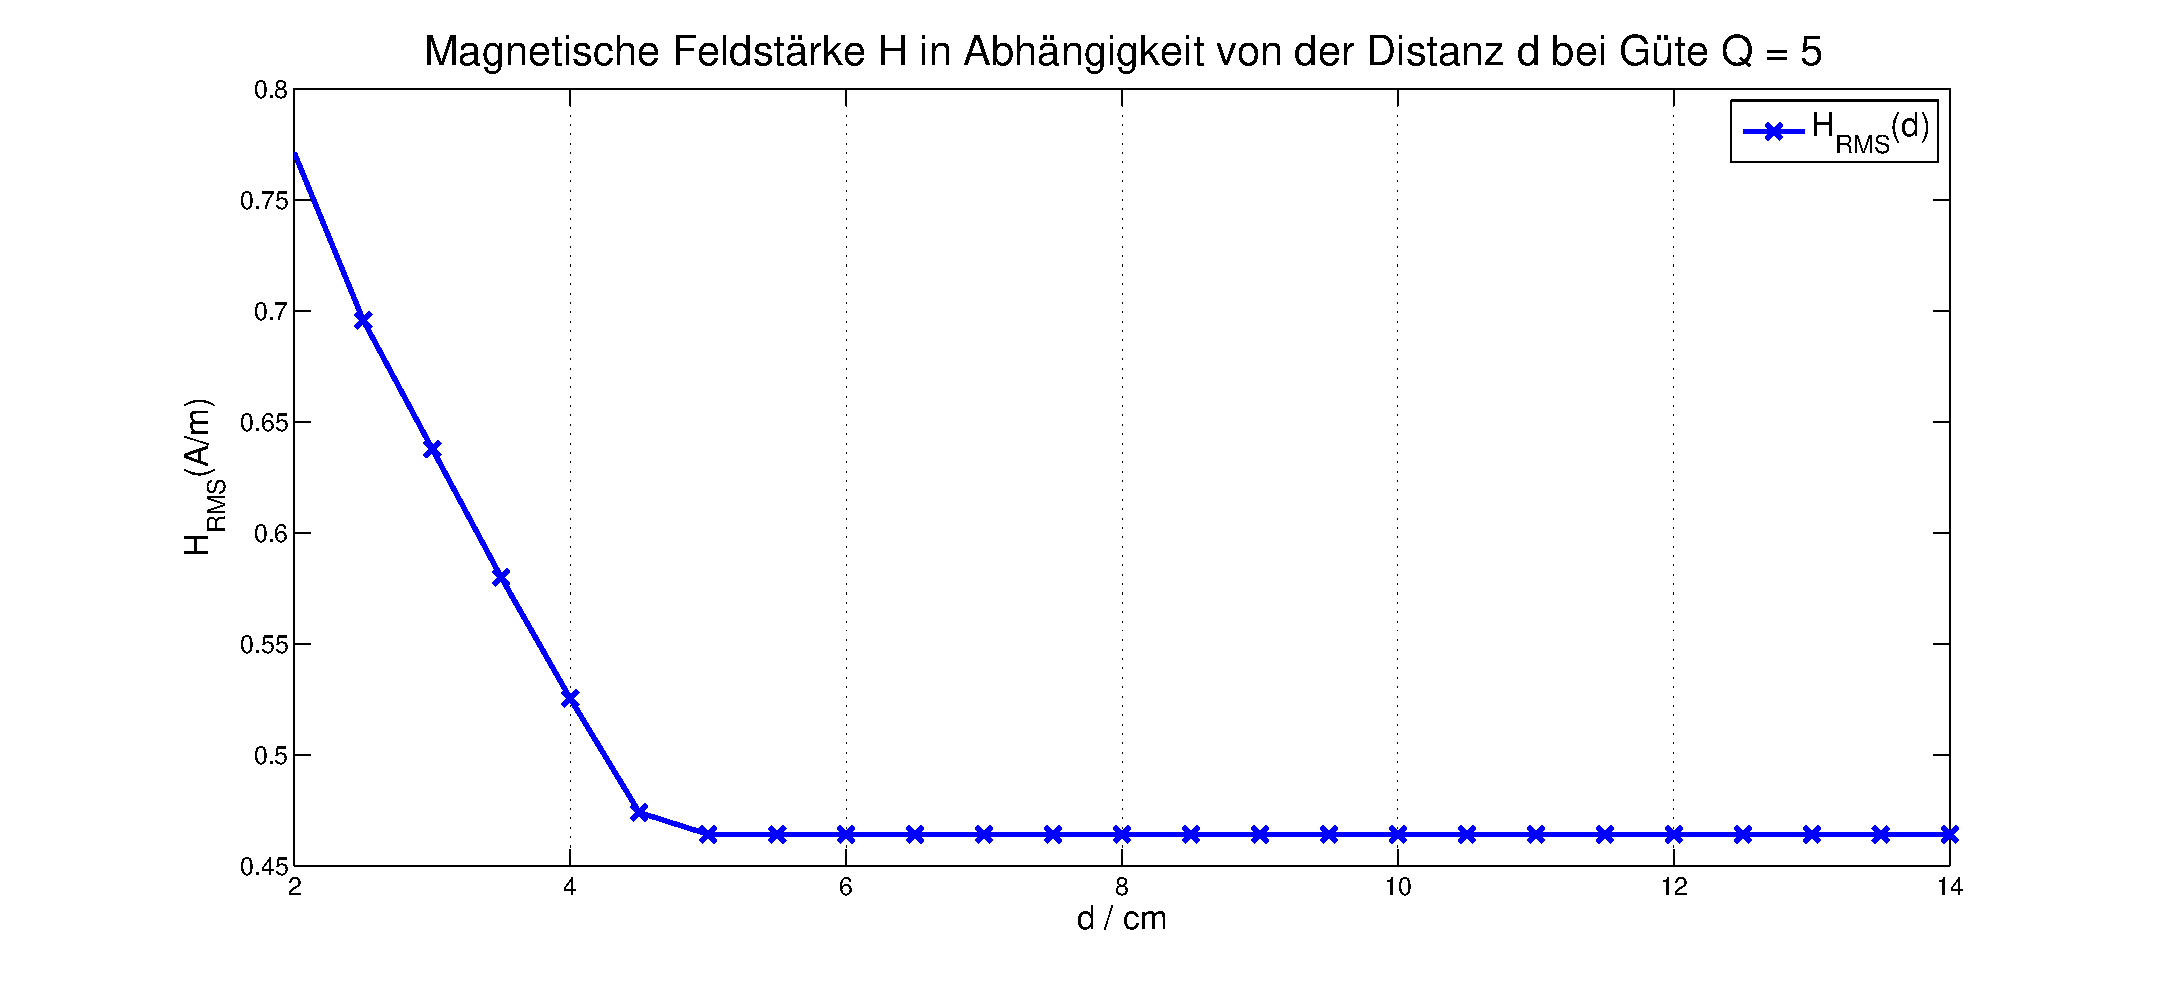
\includegraphics[width=0.9\textwidth]{figures/a1_q5.eps} 
\caption{Verlauf der Feldstärke über die Entfernung für Q = 5 und Q = 10}
\label{fig:1_q5}
\end{figure}

\subsection{Diskussion}

\section{Seitenbandpegel der Rückmodulation}
\subsection{Aufgabenstellung}

\begin{itemize}
\item???.
\end{itemize}


\subsection{Messaufbau}

\subsection{Tabellen}
\begin{table}
\begin{center}
\begin{tabular}{ |c|c|c| }
  \hline

    H(rms)) & $U_i(pp)_{oberes Seitenband}$ & $U_i(pp)_{unteres Seitenband}$\\

	[A/m] & [mV] & [mV] \\
  \hline
  $0.997$ & $320.6$ & $41.95$\\
  \hline
  $1.9984$ & $866.21$ & $727.24$ \\
  \hline
  $3.003$ & $158.54$ & $32.35$\\
  \hline
  $4.0295$ & $218.7$ & $312.14$\\
    \hline
  $5.0123$ & $175.37$ & $61.54$\\
    \hline
  $6.0388$ & $323.9$ & $267.93$ \\
    \hline 
\end{tabular}
\caption{Test}
\end{center}
\end{table} 
\subsection{Formeln}

\subsection{Berechnungsbeispiele}

\subsection{Diagramme}
%\begin{figure}[H]
%\centering
%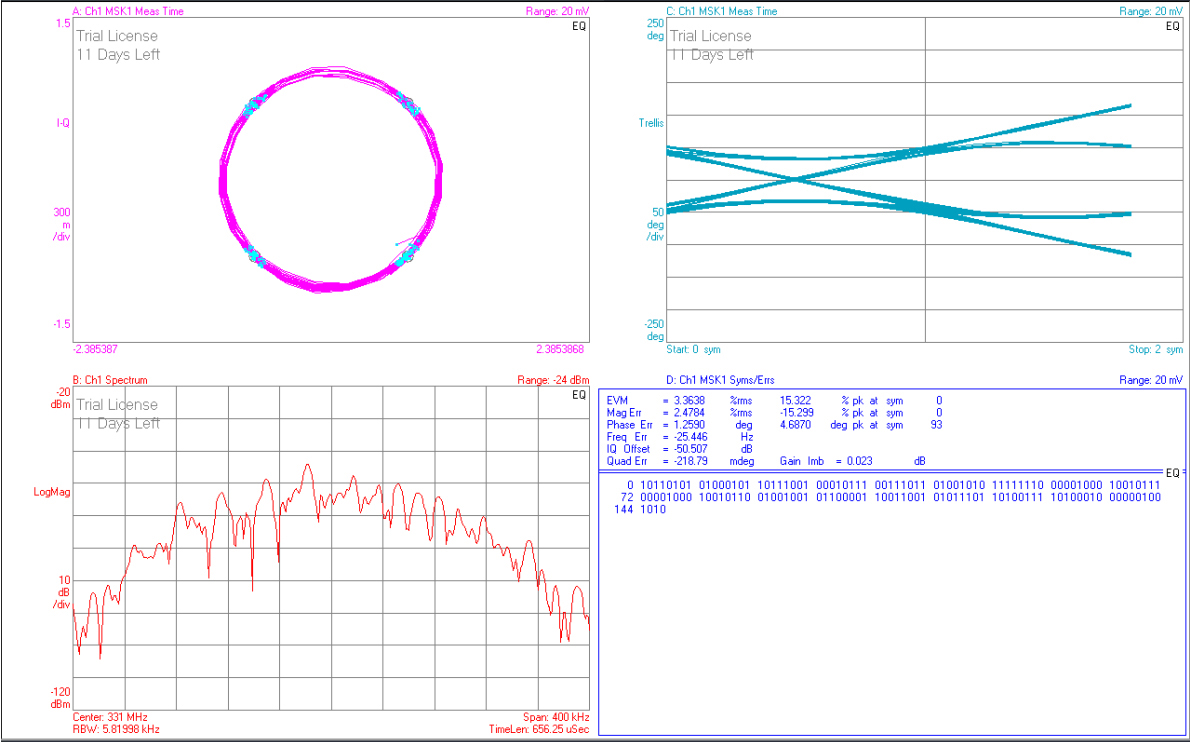
\includegraphics[width=0.9\textwidth]{figures/Aufgabe4_demod.jpg} 
%\caption{Konstellationsdiagramm, Trellis-Eye, Spektrum, Kennwerte des demodulierten GSM-Signals}
%\label{fig:a4demod}
%\end{figure}

\subsection{Diskussion}

\begin{thebibliography}{9}

\bibitem{skript}
  Markus Lenzhofer, Paul Meissner, Dr. Klaus Witrisal.
  \emph{Übung E: Messungen an digitalen Übertragungssystemen}.
  Technische Universität Graz.

\end{thebibliography}


 



   
\end{document}